\section{Experiments}

\subsection{Experiment 1: Overall Evaluation} 
In this experiment, we obtain structured data from the internal
parametric knowledge of the LLM. We evaluate the performance of the variants of Galois against
the NL, SQL, and Galois baselines, using llama-3.3-70b-instruct. The datasets used are FLIGHT-2, FLIGHT-4, GEO, MOVIES, PRESIDENTS, WORLD excluding PREMIER and FORTUNE.
A threshold \texttt{\texttau = 0.6} is used for Physical Plan selection.
The results comparison between our implementation and the former Galois paper is shown in the following tables:

\begin{table}[H]
\centering
\begin{tabular}{lcccccc}
\hline
\textbf{Metric} & \textbf{NL} & \textbf{SQL} & \textbf{Galois$_{WO}$} & \textbf{Galois$_S$} & \textbf{Galois$_A$} & \textbf{Galois$_F$} \\
\hline
F1-Cell        & 0.237 & 0.431 & 0.518 & 0.480 & 0.543 & \textbf{0.563} \\
Cardinality    & 0.462 & 0.659 & 0.691 & 0.655 & 0.799 & \textbf{0.835} \\
Tuple Constr.  & 0.065 & 0.351 & 0.389 & 0.365 & 0.448 & \textbf{0.464} \\
Avg-Score      & 0.254 & 0.481 & 0.531 & 0.500 & 0.592 & \textbf{0.622} \\
\#Tokens (M)   & 0.83  & \textbf{0.33} & 19.71 & 0.96 & 0.95 & 1.72 \\
Avg Time       & 120   & 61.4  & 1460  & 130  & 120.5 & \textbf{47.4} \\
\hline
\end{tabular}
\caption{GALOIS Paper}
\label{tab:galois_comparison}
\end{table}

\begin{table}[H]
\centering
\begin{tabular}{lcccccc}
\hline
\textbf{Metric} & \textbf{NL} & \textbf{SQL} & \textbf{Galois$_{WO}$} & \textbf{Galois$_S$} & \textbf{Galois$_A$} & \textbf{Galois$_F$} \\
\hline
F1-Cell        & 0.271 & 0.403 & 0.157 & \textbf{0.434} & 0.417 & 0.319 \\
Cardinality    & 0.500 & 0.465 & 0.357 & \textbf{0.6667} & 0.614 & 0.528 \\
Tuple Constr.  & 0.091 & 0.197 & 0.060 & \textbf{0.297} & 0.279 & 0.166 \\
Avg-Score      & 0.287 & 0.355 & 0.191 & \textbf{0.466} & 0.436 & 0.338 \\
\#Tokens (M)   & 0.005 & 0.008 & \textbf{0.163} & 0.088 & 0.076 & 0.142 \\
Avg Time       & 2.206   & 5.263  & \textbf{43.103}  & 17.952  & 24.481 & 26.196 \\
\hline
\end{tabular}
\caption{Our implementation}
\label{tab:galois_comparison}
\end{table}


\subsection{Experiment 2: Logical and Physical Optimization Impact}

This experiment evaluates the effectiveness of the logical and physical optimization strategies adopted by \textsc{GALOIS}, following the methodology described in Sections~4 and~5 of the original paper. 
The goal is to isolate and quantify how different execution strategies affect result quality, measured through the \textbf{AVG-Score} (average of F1-Cell, Cardinality, and Tuple Constraint).

\vspace{0.5em}
\noindent
All experiments are conducted on the \textbf{GEO} dataset, which queries the internal parametric knowledge of the LLM and includes 32 SQL queries with pre-computed ground truth.

\paragraph{Physical Optimization.}
At the physical level, \textsc{GALOIS} selects how data is retrieved from the LLM. 
For each query, we compare three execution strategies:
\begin{itemize}
    \item \textbf{Table-Scan}: retrieves full tuples in a single scan, providing broader context to the LLM.
    \item \textbf{Key-Scan}: first retrieves key values and then populates remaining attributes, using a chain-of-thought style interaction.
    \item \textbf{AUTO}: lets \textsc{GALOIS} automatically choose between Table-Scan and Key-Scan based on the confidence estimator described in the paper.
\end{itemize}

We report both the average result quality and the total token consumption. 
Additionally, we evaluate the \emph{AUTO accuracy}, i.e., how often the automatically selected strategy matches the best-performing fixed strategy (Table-Scan or Key-Scan) for a given query.

\begin{table}[ht]
    \centering
    \caption{Physical optimization results on GEO (AVG-Score and token usage).}
    \label{tab:exp2-physical}
    \resizebox{0.75\textwidth}{!}{
    \begin{tabular}{lcc}
        \toprule
        \textbf{Strategy} & \textbf{AVG-Score} & \textbf{Tokens (M)} \\
        \midrule
        Table-Scan & \textbf{0.315} & 0.030 \\
        Key-Scan   & 0.272 & 0.033 \\
        AUTO       & 0.274 & 0.031 \\
        \bottomrule
    \end{tabular}}
\end{table}

The results show that, on GEO, \textbf{Table-Scan achieves the highest average quality}, suggesting that richer contextual prompts help the LLM retrieve more complete and accurate data.
The AUTO strategy closely follows the best fixed plan, confirming that the confidence-based physical planner behaves robustly, although the gain over Table-Scan is limited for this dataset.

\paragraph{Logical Optimization.}
To isolate the impact of logical planning decisions, we fix the physical strategy to \textbf{Table-Scan} and evaluate different predicate pushdown strategies, as described in the paper:
\begin{itemize}
    \item \textbf{NO-PUSH}: no conditions are pushed down into the LLMScan.
    \item \textbf{PUSH-ALL} (\textsc{GALOIS\textsubscript{A}}): all WHERE conditions are pushed down.
    \item \textbf{PUSH-CONFIDENT} (\textsc{GALOIS\textsubscript{F}}): only conditions selected by the confidence estimator are pushed down.
\end{itemize}

Only queries with at least two WHERE conditions are considered, in accordance with the experimental protocol of the original work.

\begin{table}[ht]
    \centering
    \caption{Logical optimization results on GEO with fixed Table-Scan.}
    \label{tab:exp2-logical}
    \resizebox{0.75\textwidth}{!}{
    \begin{tabular}{lcc}
        \toprule
        \textbf{Strategy} & \textbf{AVG-Score} & \textbf{Tokens (M)} \\
        \midrule
        NO-PUSH                 & 0.318 & 0.015 \\
        GALOIS A (push all)     & 0.274 & 0.009 \\
        GALOIS F (confident)   & \textbf{0.397} & 0.014 \\
        \bottomrule
    \end{tabular}}
\end{table}

The results clearly show that \textbf{confidence-based pushdown (\textsc{GALOIS\textsubscript{F}})} significantly outperforms both NO-PUSH and PUSH-ALL strategies.
This confirms the key intuition of the paper: pushing all predicates may reduce cost but often degrades result quality due to increased reasoning complexity for the LLM, while selectively pushing only confident predicates yields a better balance between precision and recall.

\paragraph{Comparison with the Paper.}
Our findings are fully consistent with the original GALOIS results.
In particular, we observe the same qualitative trends:
\begin{itemize}
\item \textbf{(i)} Table-Scan can outperform Key-Scan when additional context improves factual retrieval, and
\item \textbf{(ii)} confidence-driven logical optimization (\textsc{GALOIS\textsubscript{F}}) consistently achieves the best AVG-Score among logical strategies.
\end{itemize}
These results further validate the robustness of the GALOIS optimization framework across datasets and implementations.


\subsection{Experiment 3: Impact of LLM Parameters}

This section presents a study designed to evaluate how the choice of Large Language Model (LLM) and its parameter size influences the performance of the \textsc{Galois} system. We tested the framework using three distinct models: GPT-4o \textsc{mini}, LLaMA 3.1 8B (instruct), and LLaMA 3.3 70B (instruct). 
\\\\
The primary objective was to assess whether the increased reasoning capabilities and parametric knowledge of larger models are essential for the effective execution of the logical and physical optimizations proposed in \textsc{Galois}. Furthermore, we investigated the reliability of the models' confidence scores (logprobs) as a mechanism for filtering results, aiming to balance precision and recall. 
\\\\
Performance is measured using the \textsc{Avg-Score}, comparing the fully optimized system (\textsc{Galois}$_{F}$) against simpler variants (\textsc{Galois}$_{WO}$, \textsc{Galois}$_{A}$) and standard baselines (NL and SQL).

\begin{table}[H]
    \centering
    \caption{AVG-Score of different LLMs (GALOIS PAPER)}
    \begin{tabular}{lccccc}
        \toprule
        \multicolumn{1}{c}{LLM} & NL & SQL & \textsc{Galois}$_{WO}$ & \textsc{Galois}$_{A}$ & \textsc{Galois}$_{F}$ \\
        \midrule
        GPT-4o \textsc{mini} & 0.258 & 0.240 & 0.456 & 0.457 & \textbf{0.468} \\
        LLaMA 3.1 8B         & 0.230 & 0.372 & 0.375 & 0.520 & \textbf{0.528} \\
        LLaMA 3.1 70B        & 0.254 & 0.481 & 0.531 & 0.592 & \textbf{0.622} \\
        \bottomrule
    \end{tabular}
\end{table}

\begin{table}[H]
    \centering
    \caption{AVG-Score of different LLMs (OUR RUNS)}
    \begin{tabular}{lccccc}
        \toprule
        \multicolumn{1}{c}{LLM} & NL & SQL & \textsc{Galois}$_{WO}$ & \textsc{Galois}$_{A}$ & \textsc{Galois}$_{F}$ \\
        \midrule
        GPT-4o \textsc{mini} & 0.073 & 0.295 & 0.013 & 0.298 & \textbf{0.166} \\
        LLaMA 3.1 8B         & 0.268 & 0.372 & 0.189 & 0.376 & \textbf{0.189} \\
        LLaMA 3.1 70B        & 0.287 & 0.355 & 0.191 & 0.436 & \textbf{0.338} \\
        \bottomrule
    \end{tabular}
\end{table}

\subsubsection{Discussion of Results}
The comparison between the reference benchmarks and our reproduction runs highlights several critical divergences regarding the efficacy of the optimization pipeline. In the original paper, there is a constant and continuous improvement as model size increases and as optimizations are applied. Specifically, \textsc{Galois}$_{F}$ is always the superior configuration, reaching an AVG-Score of 0.622 with LLaMA 3.1 70B.
\\\\
However, our reproduction data suggests a regression in full optimization. Unlike the reference paper, where \textsc{Galois}$_{F}$ provides the best results, our experiments show that \textsc{Galois}$_{F}$ consistently underperforms compared to \textsc{Galois}$_{A}$. This indicates that the additional logic in the full pipeline—likely the dynamic switching to the \textit{Key-Scan} operator or the confidence-based plan selection—is introducing errors rather than resolving them. Additionally, the baseline performance of the unoptimized \textsc{Galois}$_{WO}$ yields significantly lower scores in our runs compared to the paper. This suggests that the fundamental iterative retrieval mechanism without pushdown conditions is struggling to retrieve relevant tuples in our setup.

\subsubsection{Confidence Estimation Analysis}

\begin{figure}[H]
    \centering
    \begin{minipage}{0.48\textwidth}
        \centering
        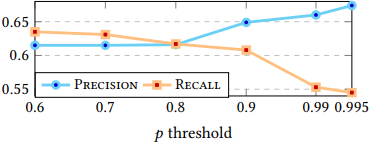
\includegraphics[width=\linewidth]{images/Galois_exp_3.png}
        \caption{Original Paper Results}
        \label{fig:galois_original_exp3}
    \end{minipage}\hfill
    \begin{minipage}{0.48\textwidth}
        \centering
        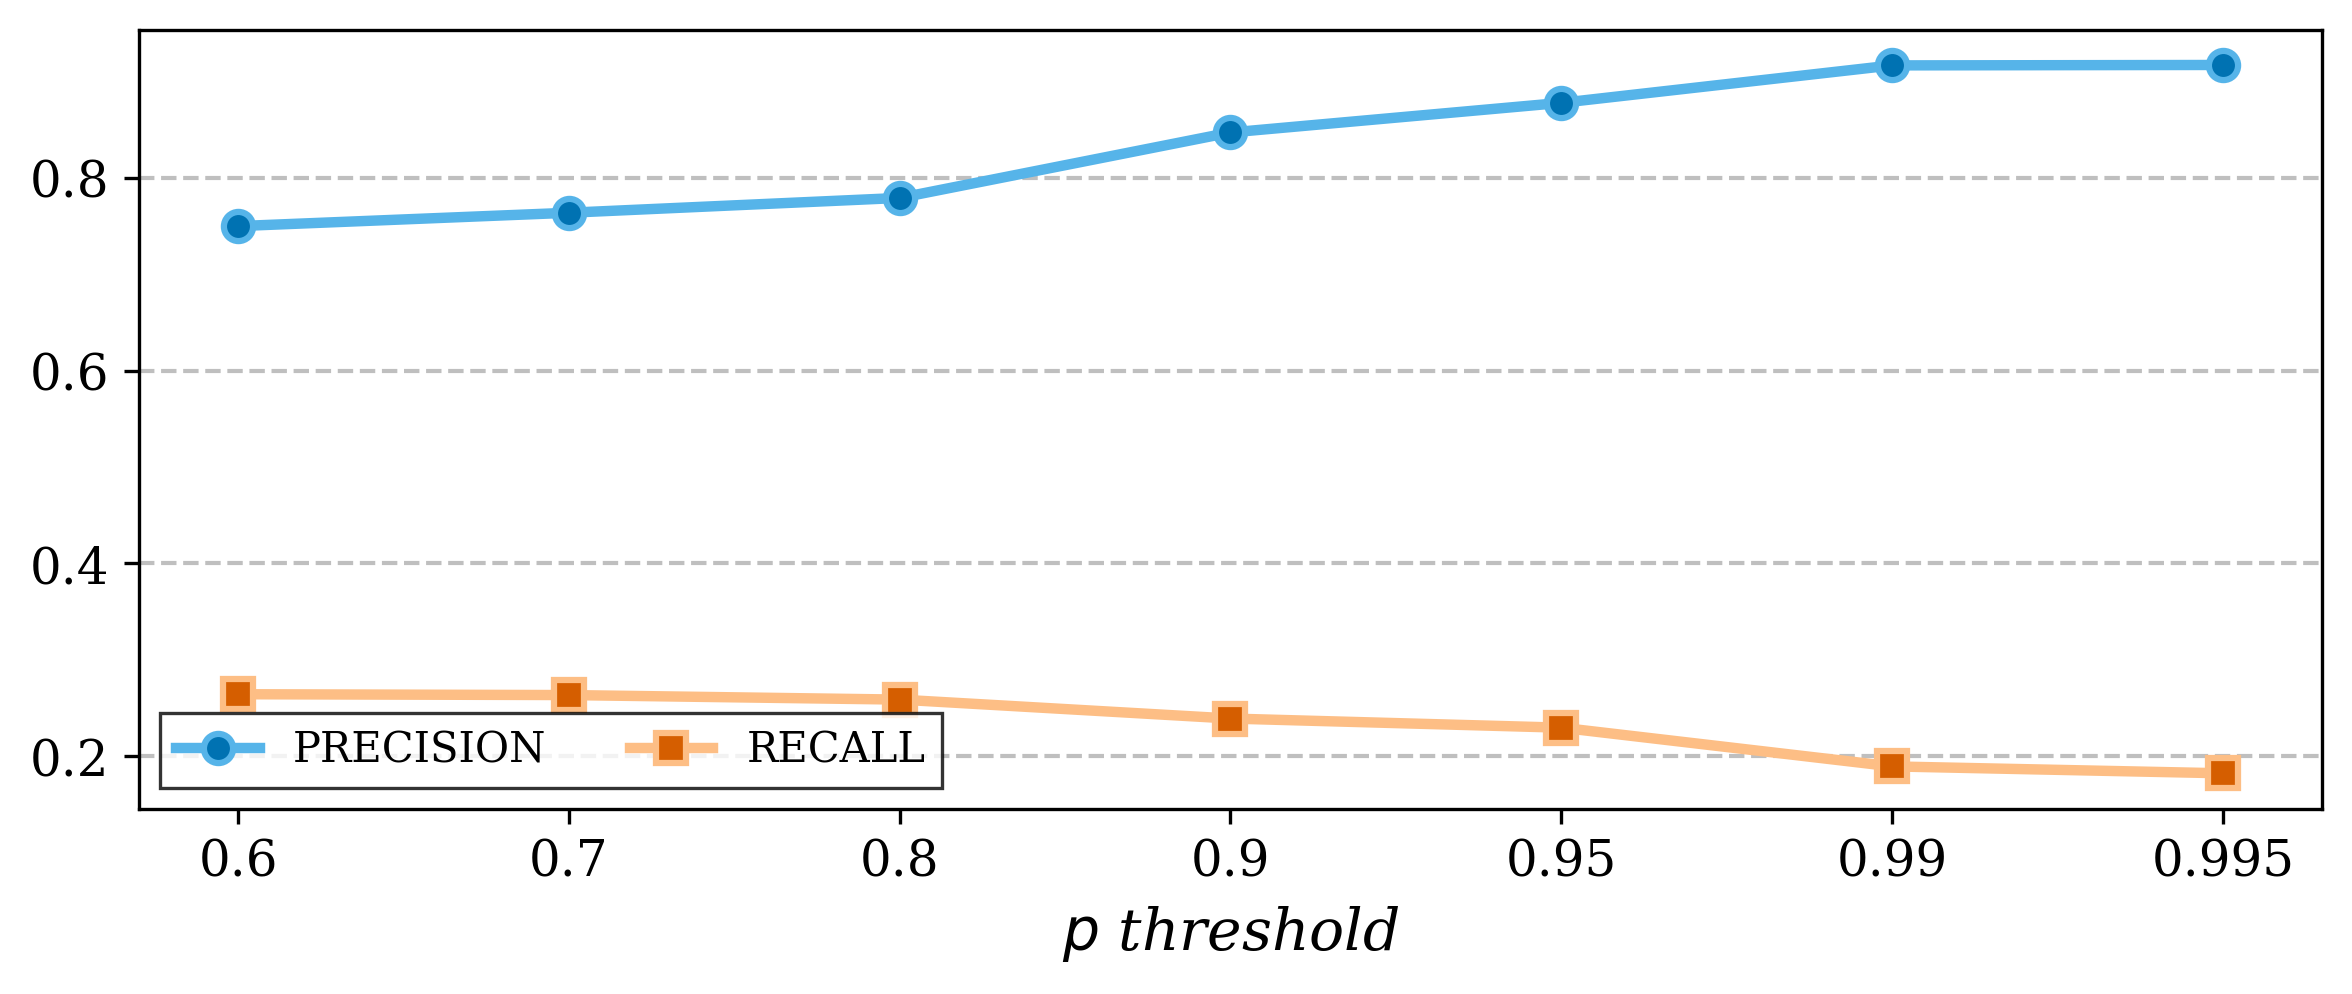
\includegraphics[width=\linewidth]{images/exp-3.png}
        \caption{Our Reproduction Results}
        \label{fig:our_exp3}
    \end{minipage}
\end{figure}

The results in Figure \ref{fig:our_exp3} confirm the expected trade-off: as the threshold $p$ increases from 0.6 to 0.995, the \textbf{Precision} improves notably in our runs, rising from approximately 0.75 to over 0.90. This demonstrates that the model's internal confidence is a reliable proxy for the factual correctness of the generated data; when the model is confident, the data is likely correct.
\\\\
However, the charts also reveal the root cause of the lower overall scores observed in Table 2. While the original paper (left) shows \textbf{Recall} starting above 0.60, our reproduction (right) shows Recall starting at a very low baseline (approximately 0.26 at $p=0.6$). Even with lenient filtering, the system retrieves less than 30\% of the expected tuples. This low initial recall explains why the AVG-Scores in our reproduction are capped: even if precision is high, the system simply fails to extract the majority of the required information from the model's parametric knowledge.


\subsection{Experiment 4: Impact of retrieved values}

Here we implemented an automated evaluation pipeline  ("Impact of Rarity and Temporality"), focusing on the \textbf{PRESIDENTS} domain. The primary objective is to quantify how the frequency of data in pre-training (popularity) and its temporal recency influence the ability of Large Language Models (LLMs)  to measure two specific biases.
\begin{itemize}
    \item \textbf{Rarity}: Compares performance on popular entities (USA) versus rare entities (Venezuela).
    \item \textbf{Temporality}: Compares performance on recent events versus historical events . For this purpose we split the queries into three categories: ALL-TIME covering all dates, RECENT for queries that cover data from late 1900 to today, and PAST for queries
for data till the late 1900.
\end{itemize}



By benchmarking model modalities (GALOIS, NL, SQL) against the Ground Truth, the script calculates the AVG-SCORE. The results confirm that query generation quality degrades significantly when dealing with rare or historical data, as we can see in the tables below:

\begin{table}[ht]
    \centering
    \caption{Experimental Results: Impact of Rarity and Temporality on Query Execution Quality (AVG-SCORE).}
    \label{tab:combined_results}
    \begin{tabular}{lcccccc}
        \toprule
        \textbf{Category} & \textbf{GALOIS\textsubscript{A}} & \textbf{GALOIS\textsubscript{F}} & \textbf{GALOIS\textsubscript{S}} & \textbf{GALOIS\textsubscript{WO}} & \textbf{NL} & \textbf{SQL} \\
        \midrule
        \multicolumn{7}{l}{\textit{Impact of Rarity (Country)}} \\
        \midrule
        Presidents-USA & 0.570 & \textbf{0.652} & 0.587 & 0.089 & 0.352 & 0.320 \\
        Presidents-Venezuela & 0.282 & 0.212 & \textbf{0.323} & 0.051 & 0.091 & 0.257 \\
        \midrule
        \multicolumn{7}{l}{\textit{Impact of Temporality}} \\
        \midrule
        Recent & \textbf{0.532} & 0.531 & 0.449 & 0.095 & 0.375 & 0.318 \\
        Past & 0.240 & 0.305 & \textbf{0.378} & 0.000 & 0.183 & 0.281 \\
        All-Time & 0.427 & 0.420 & \textbf{0.479} & 0.077 & 0.160 & 0.277 \\
        \bottomrule
    \end{tabular}
\end{table}


\subsection{Experiment 5: Impact of SQL Query Complexity on Retrieval Quality}
\textbf{Objective}: The objective of this experiment is to evaluate the robustness and stability of the GALOIS system as the structural and logical complexity of the input SQL query varies. Since Large Language Models (LLMs) tend to degrade in performance when handling complex logic (such as multiple joins or nested aggregations).
\\\textbf{Methodology and Query Taxonomy}: To conduct this analysis, we implemented a static classifier (\texttt{classify\_query\_complexity}) that parses the Abstract Syntax Tree (AST) of each SQL query via \texttt{sqlglot} and assigns it to one of six mutually exclusive complexity categories, ordered by expected difficulty:
\begin{itemize}
    \item \textbf{SP2 (Selection-Projection Simple)}: Linear queries involving only selection and projection operations with at most 2 conditions in the \texttt{WHERE} clause. These represent the simplest base case.
    \item \textbf{SP2> (Selection-Projection Complex)}: Selection/projection queries featuring more than 2 filtering conditions, requiring the LLM to manage a denser logical context.
    \item \textbf{DIST (Distinct)}: Queries including the DISTINCT clause, requiring the system to handle explicit result deduplication.
    \item \textbf{AGGR (Aggregation)}: Queries utilizing aggregation functions (COUNT, SUM, AVG, MAX, MIN), which require arithmetic reasoning or counting capabilities on retrieved tuples.
    \item \textbf{G/O (Group By / Order By)}: Queries imposing sorting or grouping of data, testing the system's ability to structure output sequentially.
    \item \textbf{JOIN}: Queries involving joins between two or more tables. This is considered the most complex category, as it requires the system to decompose the problem into multiple scans (multi-table retrieval) and reconstruct relationships in local post-processing.
\end{itemize}
The GALOIS results are compared against the Ground Truth (loaded from pre-calculated JSON files) using three metrics: F1-Cell Exact, Cardinality, and Tuple Constraint of the \texttt{galois\_eval.py} script.
In Figure \ref{fig:exp5-avg} we compare metrics of our run with the GALOIS paper ones and is clear that JOIN operations are worsening the results.
The main reason for that is the difficulty of LLM to retrieve results that match the queries with JOIN clause, something already seen in the GALOIS results in Section \ref{results_galois}.
Instead figure \ref{fig:exp5-tokens} shows the token usage of our run compared to the GALOIS paper ones.


\begin{figure}[H]
    \centering
    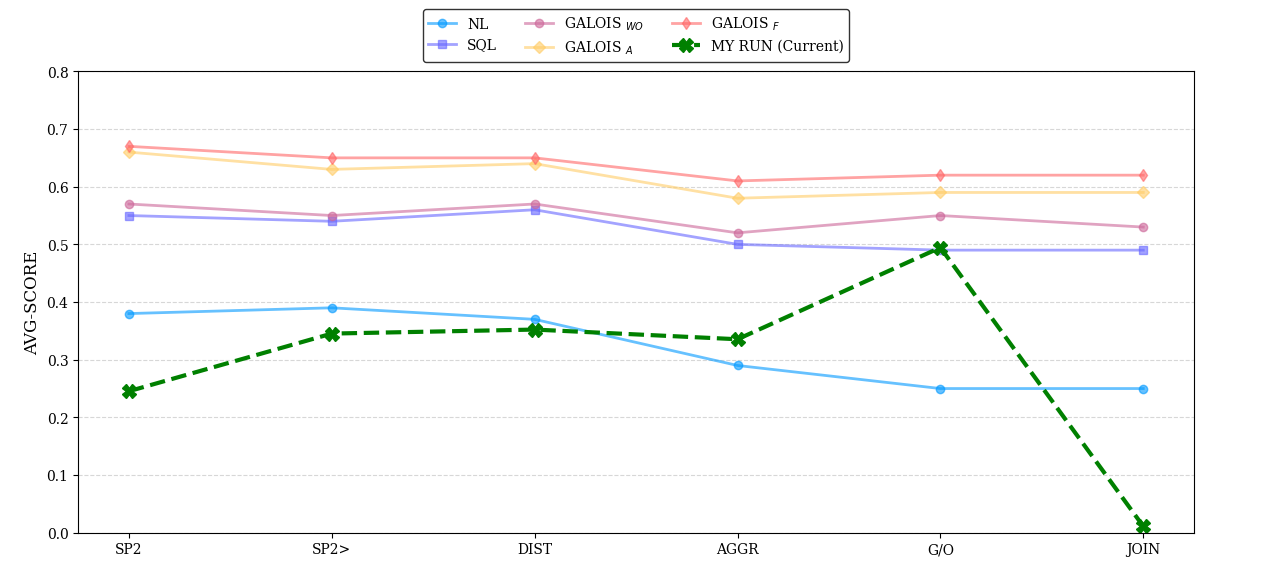
\includegraphics[width=0.9\textwidth]{images/exp-5-avg.png}
    \caption{Result quality w.r.t query complexity}
    \label{fig:exp5-avg}
\end{figure}

\begin{figure}[H]
    \centering
    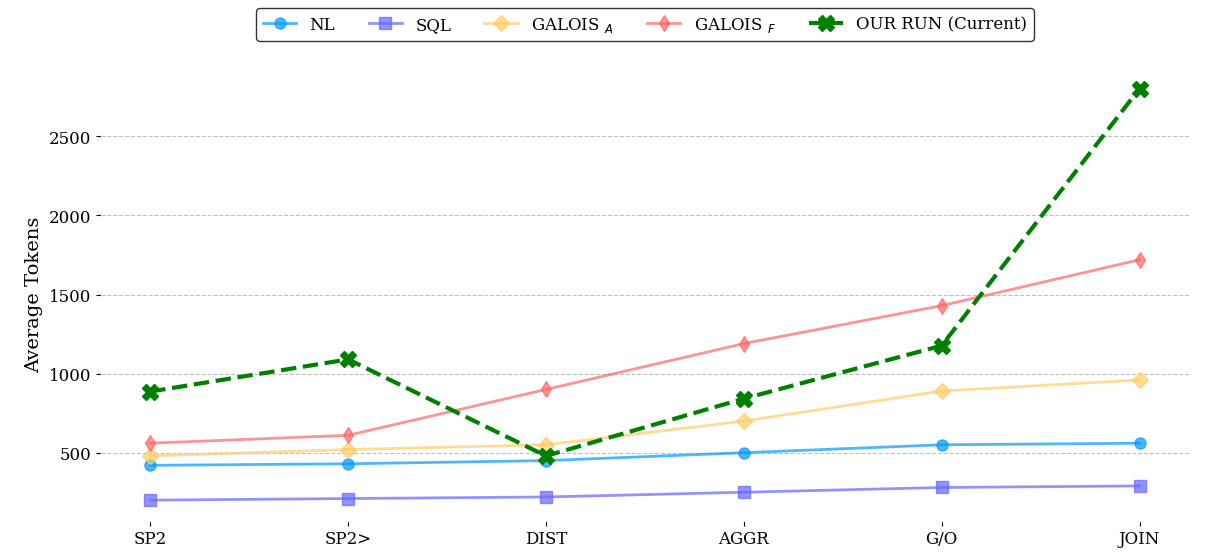
\includegraphics[width=0.9\textwidth]{images/exp-5-tokens.png}
    \caption{Costs w.r.t query complexity. Galois WO (not reported)}
    \label{fig:exp5-tokens}
\end{figure}






\subsection{Experiment 6: Evolution of Prompt Size}

The goal is to evaluate how logical optimizations impact both the prompt size and the number of iterations required to answer a query.
For every query in the Internal Knowledge (IK) datasets, this task executes three distinct configurations of the system, all fixed to use the Table-Scan physical strategy.
The first configuration is \textbf{GALOIS $\emptyset$ (No-Push)}, which serves as the unoptimized baseline where no conditions are pushed to the LLM. The second is \textbf{GALOIS A (Push-All)}, an aggressive optimization that pushes all WHERE conditions into the prompt. The third is \textbf{GALOIS F}, the confidence-based approach that selectively pushes only high-confidence conditions.
For each run, the script logs the total number of input tokens, the number of iterations performed, and whether the execution converged within the maximum limit of 10 iterations.

The results from this replication, conducted using llama-3.3-70b-instruct, align closely with the findings of the original paper, confirming the significant efficiency gains provided by the optimizations. The baseline GALOIS $\emptyset$ proves to be the most resource-intensive approach in terms of tokens and time consuming. 
Furthermore, this unoptimized strategy exhibits stability issues, failing to converge for 11 queries within the iteration limit. Conversely, applying logical optimizations drastically improves performance. GALOIS A reduces the average token count and the iterations, successfully eliminating all convergence failures. 
GALOIS F achieves the best overall efficiency, further lowering the token usage and the average iterations. These findings demonstrate that pushing filter conditions down to the LLM not only reduces the volume of data processed but also creates a more robust and faster extraction process, preventing the model from getting stuck in long retrieval loops.

\begin{table}[h]
    \centering
    \caption{Prompt size without push-down (Galois $\emptyset$ ) and with Galois’s optimizations.}
    \label{tab:exp6-prompt-size}
    \begin{tabularx}{\textwidth}{l >{\centering\arraybackslash}X >{\centering\arraybackslash}X >{\centering\arraybackslash}X}
        \toprule
        \textbf{Method} & \textbf{AVG \# INPUT TOKENS} & \textbf{AVG \# ITERATIONS} & \textbf{\# QUERIES $\ge$ MAX\_ITER} \\
        \midrule
        GALOIS $\emptyset$ (No-Push) & 1301 & 5.05 & 11 \\
        GALOIS A (Push-All)         & 1100 & 3.31 & \textbf{0} \\
        GALOIS F             & \textbf{1090} & \textbf{3.26} & \textbf{0} \\
        \bottomrule
    \end{tabularx}
    
    \vspace{0.1cm}
    \footnotesize
    \textit{Note: Results aggregated over 77 queries from IK datasets.}
\end{table}

\newpage

\subsection{Experiment 7: Threshold Setup}
This experiment focuses on calibrating the confidence threshold parameter, denoted as $\tau$, which governs the \textsc{Galois} physical optimizer. The system uses this threshold to dynamically choose between two physical operators: \textit{Table-Scan} (retrieving full tuples with broader context) and \textit{Key-Scan} (iterative retrieval using Chain-of-Thought reasoning).
\\\\
The selection logic dictates that if the estimated confidence of the model for the query exceeds $\tau$, \textsc{Galois} employs the \textit{Key-Scan} operator; conversely, if the confidence falls below $\tau$, the system reverts to the \textit{Table-Scan} strategy. To determine the optimal $\tau$, we executed the system on the GEO-TEST dataset (used as a calibration set to avoid overfitting on the main benchmarks) while varying $\tau$ from $1.0$ (forcing \textit{Table-Scan}) down to $0.0$ (forcing \textit{Key-Scan}). We evaluated three models: LLaMA 3.3 70B, LLaMA 3.1 8B, and GPT-4o \textsc{mini}.

\begin{figure}[H]
    \centering
    \begin{minipage}{0.48\textwidth}
        \centering
        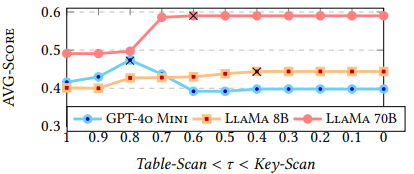
\includegraphics[width=\linewidth]{images/Galois_exp_7.png}
        \caption{Original Paper Results}
        \label{fig:galois_original_exp7}
    \end{minipage}\hfill
    \begin{minipage}{0.48\textwidth}
        \centering
        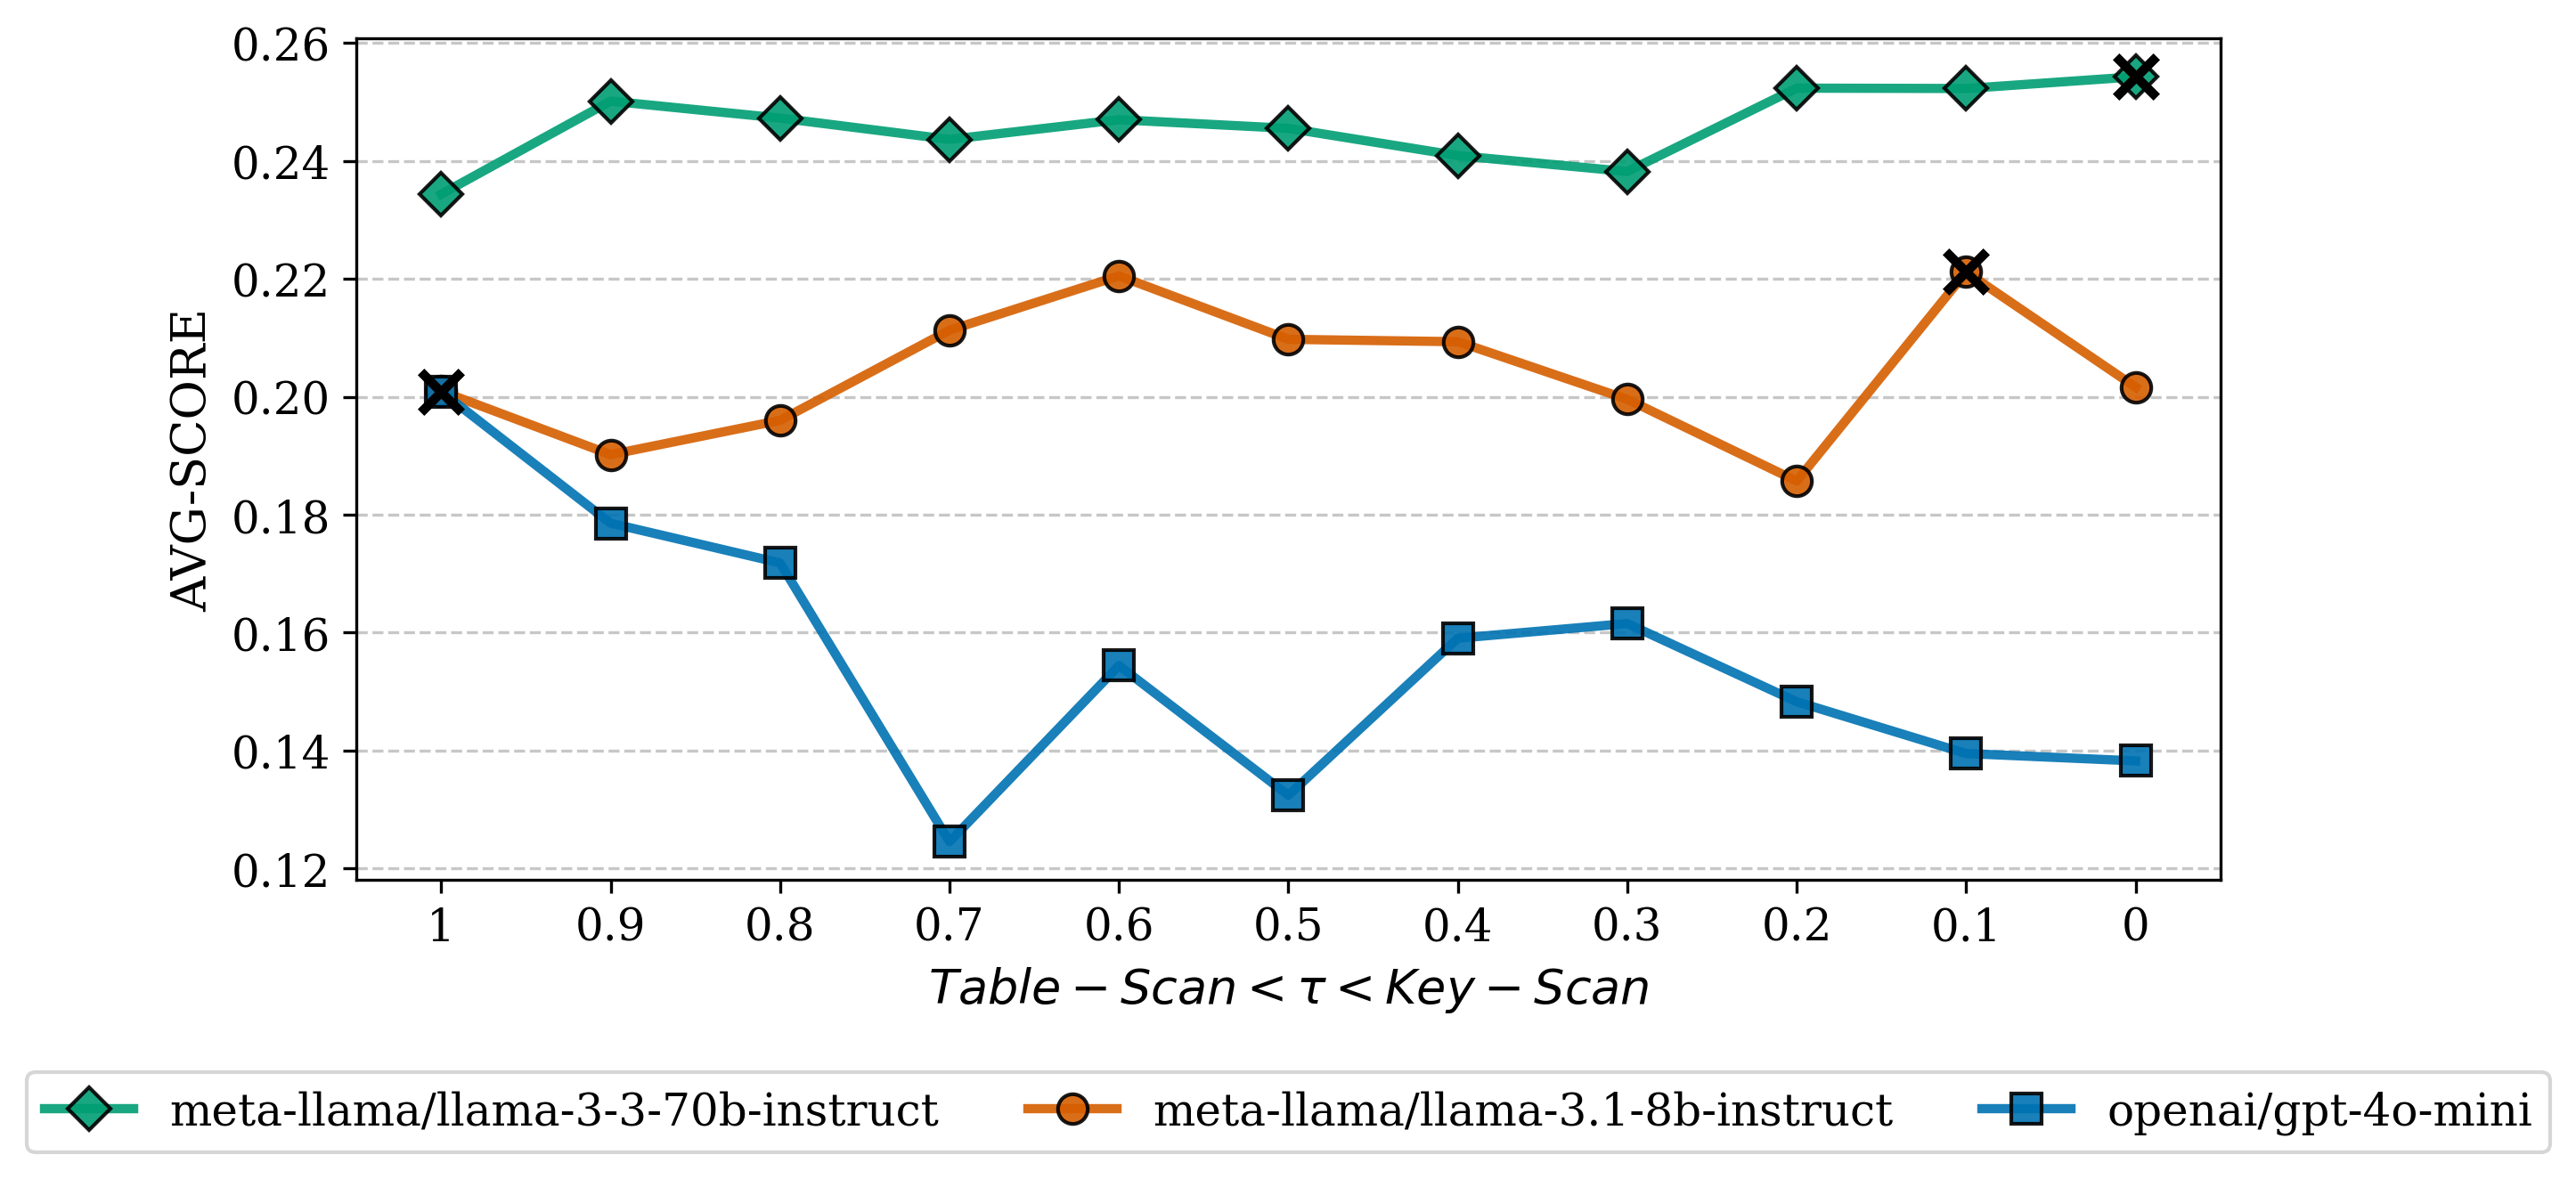
\includegraphics[width=\linewidth]{images/exp-7.png}
        \caption{Our Reproduction Results}
        \label{fig:our_exp7}
    \end{minipage}
    \label{fig:threshold_comparison}
\end{figure}

\subsubsection{Analysis of Calibration Results}

The results of our calibration runs, depicted in Figure \ref{fig:our_exp7} (right), present a distinct behavior compared to the findings in the original \textsc{Galois} paper (left).

\paragraph{Performance Discrepancy}
First, consistent with Experiment 3, the absolute performance in our runs is significantly lower. The original paper reports peak AVG-Scores between 0.4 and 0.6. In contrast, our best-performing model (LLaMA 3.3 70B) peaks at approximately 0.25, and GPT-4o \textsc{mini} peaks at 0.20.

\paragraph{Model-Specific Behavior and Optimal Thresholds}
The calibration curves reveal divergent optimal strategies for the different model sizes.\\\\
For \textbf{GPT-4o \textsc{mini}}, the curve demonstrates a negative correlation between \textit{Key-Scan} usage and quality. The highest score is achieved at $\tau=1$ (pure \textit{Table-Scan}), and performance degrades as $\tau$ decreases. This contrasts with the paper, which identified an optimal $\tau=0.8$, suggesting that the iterative \textit{Key-Scan} operator in our implementation is detrimental for this model, likely due to context fragmentation or the "zero recall" issue identified in the previous study.
\\\\
Conversely, \textbf{LLaMA 3.3 70B} exhibits the opposite behavior. Performance gradually improves as we lower the threshold, peaking at $\tau=0.1$ and $\tau=0$ (pure \textit{Key-Scan}). While the original paper found an optimal $\tau=0.6$, our data suggests that for the largest model, the \textit{Table-Scan} is insufficient, and the model relies entirely on the granular, iterative retrieval of \textit{Key-Scan} to achieve its maximum accuracy. 
\\\\
Finally, the behavior of \textbf{LLaMA 3.1 8B} is noisy, with local maxima at both $\tau=1$ and $\tau=0.1$. This inconsistency suggests that the 8B model struggles to maintain stability in either mode, making it sensitive to the specific prompt structure rather than the logical operator choice.
\\\\
In conclusion, our calibration suggests that the dynamic switching mechanism (using intermediate $\tau$ values) is less effective in our current reproduction than in the original study. The models tend to prefer binary extremes: the smaller model requires the context of \textit{Table-Scan}, while the larger model requires the reasoning steps of \textit{Key-Scan}.

\subsection{Experiment 8: Errors w.r.t. the optimal plan}
\textbf{Objective}: This experiment aims to quantify the efficacy of the \textbf{Logical Planner} (the component deciding which strategy to adopt) by measuring the "Optimality Gap". The Optimality Gap represents the performance difference between the automatic choice made by \texttt{GALOIS\_F} and the theoretical optimal choice ("Oracle") that the system could have made if it had selected the best possible strategy for every single query.
For every query present in the target datasets (GEO, WORLD, MOVIES), the runner  executes the configurations in "brute-force" mode.\\\\
\\\textbf{Oracle Definition and Gap Calculation}: For each query $q$, we define the Oracle score ($S_{opt}$) as the maximum score obtainable among the available strategies:$$S_{opt}(q) = \max(S_{GALOIS\_A}(q), S_{GALOIS\_WO}(q), S_{GALOIS\_F}(q))$$.\\ \textbf{The Optimality Gap} is calculated as the average difference between the Oracle and the adaptive variant:$$Gap = \frac{1}{N} \sum_{q \in Q} (S_{opt}(q) - S_{GALOIS\_F}(q))$$ A gap close to 0 indicates that the GALOIS\_F automatic selector is choosing the best available strategy almost every time. A high gap suggests that, although a winning strategy exists for that query (e.g., Key-Scan), the system erroneously opted for another
Results in Figure \ref{fig:exp8} report the AVG-Score on All the queries in the dataset, and we also break the AVG-Score for each dataset.

\begin{figure}[H]
    \centering
    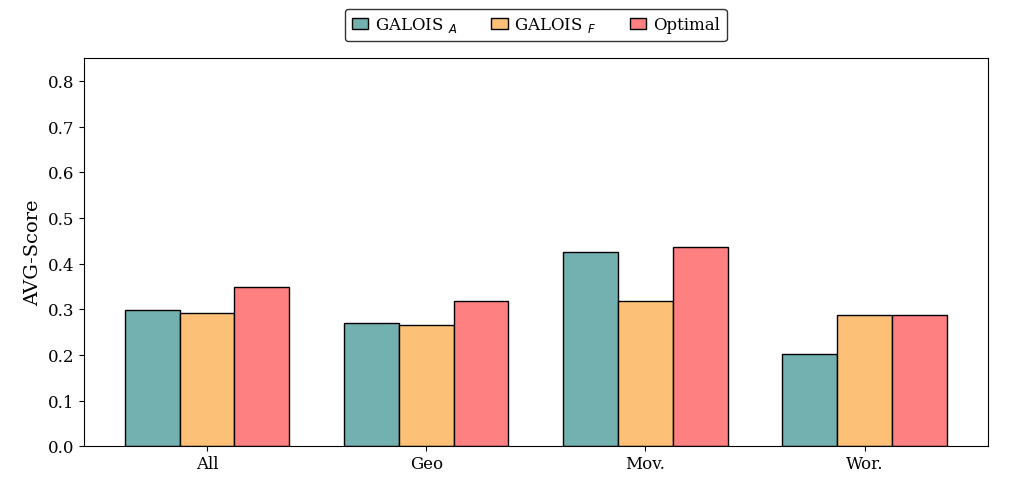
\includegraphics[width=0.9\textwidth]{images/exp-8.png}
    \caption{AVG-Score Comparison for Galois A and Galois F against the optimal plans across all datasets.}
    \label{fig:exp8}
\end{figure}